\documentclass[11pt,fleqn,twoside]{article}
\usepackage{makeidx}
\makeindex
\usepackage{palatino} %or {times} etc
\usepackage{plain} %bibliography style 
\usepackage{amsmath} %math fonts - just in case
\usepackage{amsfonts} %math fonts
\usepackage{amssymb} %math fonts
\usepackage{lastpage} %for footer page numbers
\usepackage{fancyhdr} %header and footer package
\usepackage{mmpv2} 
\usepackage{url}
\usepackage{float}

% the following packages are used for citations - You only need to include one. 
%
% Use the cite package if you are using the numeric style (e.g. IEEEannot). 
% Use the natbib package if you are using the author-date style (e.g. authordate2annot). 
% Only use one of these and comment out the other one. 
\usepackage{cite}
\usepackage[parfill]{parskip}
%\usepackage{natbib}

\begin{document}

\name{Aidan Wynne Fewster}
\userid{awf1}
\projecttitle{NHS Wales formulary and antimicrobial Android application}
\projecttitlememoir{NHS Wales Android application} %same as the project title or abridged version for page header
\reporttitle{Requirements Specification}
\version{1.0}
\docstatus{Release}
\modulecode{CS39440}
\degreeschemecode{G400}
\degreeschemename{Computer Science}
\supervisor{Andrew Starr} % e.g. Neil Taylor
\supervisorid{aos}
\wordcount{}

%optional - comment out next line to use current date for the document
%\documentdate{10th February 2014} 
\mmp

\setcounter{tocdepth}{3} %set required number of level in table of contents


%==============================================================================
\section{Introduction}
%==============================================================================
\subsection{Purpose of this document}
%==============================================================================\
This document will outline the functional, user interface and security requirements for the NHS Wales formulary and antimicrobial Android application. It will also include use cases for the system. This document can later be used during testing to ensure that the system meets all the requirements outlined within.


%==============================================================================
\subsection{Project overview}
%==============================================================================
The main focus of this project is to produce a mobile application for Android which will aid NHS medical staff in obtaining useful information for drugs which are available within the NHS . For more information refer to the Outline Specification document.


%==============================================================================
\section{Project details}
%==============================================================================
This section will describe the general factors that affect the requirements. It will describe the characteristics of the users using the system and explain how they shall be using the system. I will also outline any assumptions that I have made.

%==============================================================================
\subsection{User characteristics}
%==============================================================================
The primary users of the application will be medical staff of NHS Wales. They will be using the applications to search for information on drugs available within the NHS. They should already have broad knowledge of information displayed within the application. 

As the application will be built on the Android platform the member of staff should already be familiar with the user interface of Android and therefore be able to natively use applications that follow the Android design guidelines.

%==============================================================================
\subsection{Assumptions}
%==============================================================================
As the application will be used in hospitals I am assuming that an internet connection will not be available at all times when the application is in use therefore the data used by the application must be stored for offline use.

Another assumption I am making is that the member of staff will be installing the application on a device they are familiar with and therefore know how to use the Android operating system.

%==============================================================================
\subsection{Dependencies}
%==============================================================================
The application must have access to the NHS database in order to retrieve updates to the list of drugs. I aim to access this database through a JSON API, but I do not yet know if this is possible as I haven''t met with the NHS yet.


%==============================================================================
\section{Requirements}
%==============================================================================
\subsection{Functional requirements}
%==============================================================================
This section will list the functional requirement's (FR)'s for this project.

\begin{description}
\item[FR1] The user must be able to login to the NHS database using their credentials.
\item[FR2] The user must be able to reset their credentials should they forget them.
\item[FR3] Application must synchronise it's database with the NHS's database so that the data can be used for offline use.
\item[FR4] The user must be able to see drugs which have received updates to their information within the last 3 months.
\item[FR5] The user must be able to scroll through a list of drugs to find a drug.
\item[FR6] The user must be able to find a drug by entering part of the drugs name, the system must provide suggestions once the user begins typing.
\item[FR7] Once a user has found a drug, they should be neatly presented with the appropriate information about that drug.
\item[FR8] Once a user has found a drug, the user must be able to enter a patients weight and be presented with recommended dosage requirements for that patient.
\item[FR9] The user must receive a notification to their device when an update to a drug has been made within the NHS database.
\item[FR10] The user must be able to force the application to fetch updates from the NHS database.
\item[FR11] Developers must be able to set the structure of the database within an XML file to allow easy customisation of the application in future.
\end{description}

%==============================================================================
\subsection{User interface requirements}
%==============================================================================
The user interface for the application should follow the guidelines set out in the Android developer design guide. Following these guidelines will allow the user to learn to use the application with minimalistic effort.

When the user first opens the application, they will be presented with a login field. Upon logging in they will be presented with the latest updates to drugs and buttons. The buttons will allow the user to begin searching for a drug, force an update of the database and open the settings panel.

When the user selects a drug they will be presented with a neatly presented page with collapsible sections of information. This page will also contain a button to open the dosage calculation.

The user interface must be simplistic but make it clear what action you are currently performing. For example when calculating the dosage of penicillin for a patient, the user must be able to clearly see that penicillin has been selected and the weight of the patient used to calculate the dosage.
%==============================================================================
\subsection{Security}
%==============================================================================

The NHS have expressed concerns over the security of the data provided by the database. A number of problems will arise for the NHS should the information contained within the database be released to the public. It Is therefore fundamentally important that all data store on the device and all data transmitted to the device be encrypted.

The data stored on the device should be encrypted so that other applications can not access the information and should the device be placed in the hands of a malicious user the data should be inaccessible.

When database synchronisation occurs the data being transmitted should be transmitted over SSL so that the data is encrypted.


%==============================================================================
\section{Use case diagram}
%==============================================================================
\begin{figure}[H]
\centering
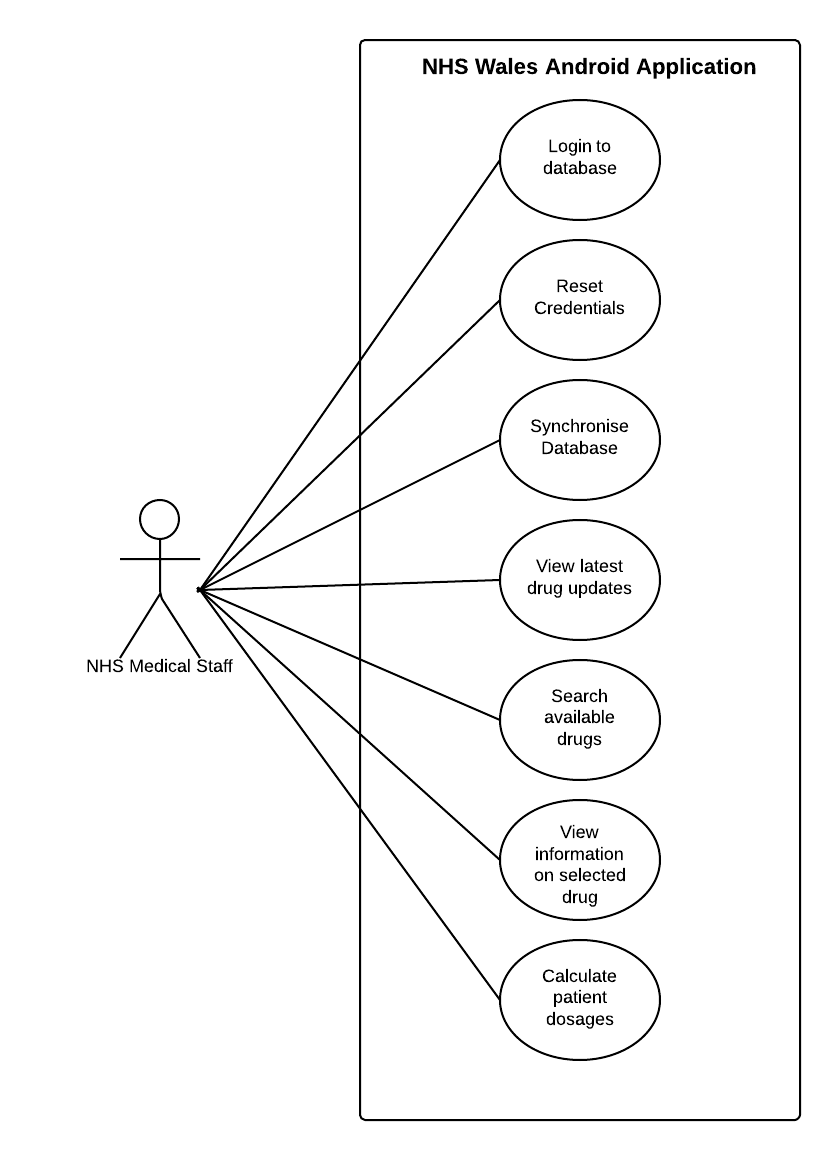
\includegraphics[width=4.4in]{useCase}
\caption{Use case diagram for the NHS application}
\end{figure}

\end{document}
